\documentclass{standalone}
\usepackage{tikz}
\usetikzlibrary{shapes.geometric, arrows.meta, positioning, calc}

\begin{document}
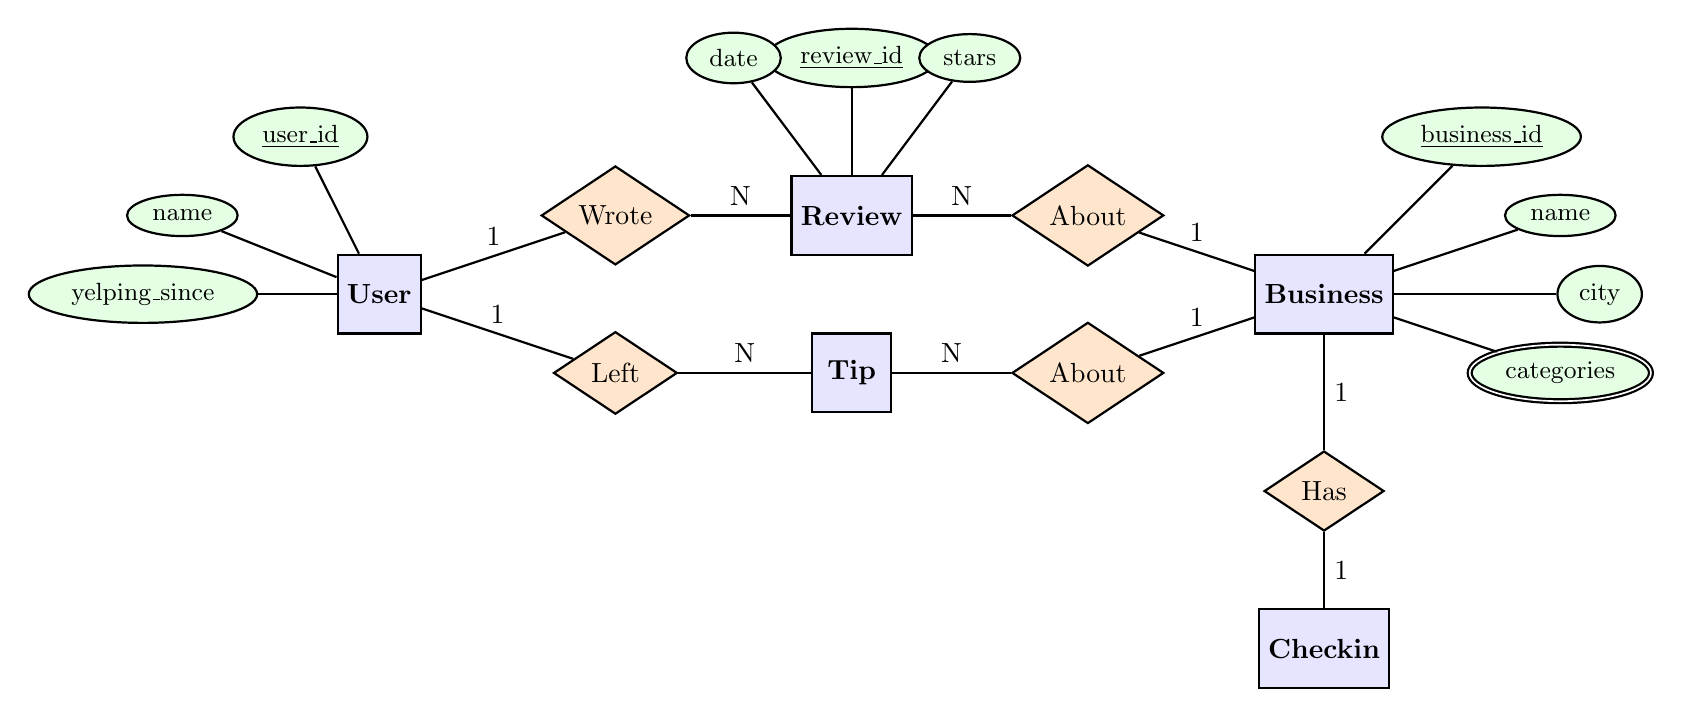
\begin{tikzpicture}[
    node distance=2.5cm and 2cm,
    entity/.style={rectangle, draw=black, thick, fill=blue!10, minimum size=1cm, align=center, font=\bfseries},
    relationship/.style={diamond, aspect=1.5, draw=black, thick, fill=orange!20, minimum size=1cm, align=center},
    attribute/.style={ellipse, draw=black, thick, fill=green!10, minimum size=0.5cm, align=center, font=\small},
    multi/.style={ellipse, draw=black, double, thick, fill=green!10, minimum size=0.5cm, align=center, font=\small},
    link/.style={-, thick}
]

% Entities & Relationships Layout
\node[entity] (user) at (0, 0) {User};
\node[relationship] (wrote_rev) at (3, 1) {Wrote};
\node[relationship] (left_tip) at (3, -1) {Left};
\node[entity] (review) at (6, 1) {Review};
\node[entity] (tip) at (6, -1) {Tip};
\node[relationship] (rev_for) at (9, 1) {About};
\node[relationship] (tip_for) at (9, -1) {About};
\node[entity] (business) at (12, 0) {Business};
\node[relationship] (has_chk) at (12, -2.5) {Has};
\node[entity] (checkin) at (12, -4.5) {Checkin};

% Paths & Cardinalities
\draw[link] (user) -- (wrote_rev) node[midway, above] {1};
\draw[link] (wrote_rev) -- (review) node[midway, above] {N};
\draw[link] (user) -- (left_tip) node[midway, above] {1};
\draw[link] (left_tip) -- (tip) node[midway, above] {N};
\draw[link] (review) -- (rev_for) node[midway, above] {N};
\draw[link] (rev_for) -- (business) node[midway, above] {1};
\draw[link] (tip) -- (tip_for) node[midway, above] {N};
\draw[link] (tip_for) -- (business) node[midway, above] {1};
\draw[link] (business) -- (has_chk) node[midway, right] {1};
\draw[link] (has_chk) -- (checkin) node[midway, right] {1};

% Key Attributes
\node[attribute] (u_id) at (-1, 2) {\underline{user\_id}};
\node[attribute] (u_name) at (-2.5, 1) {name};
\node[attribute] (u_yelp) at (-3, 0) {yelping\_since};
\draw[link] (user) -- (u_id);
\draw[link] (user) -- (u_name);
\draw[link] (user) -- (u_yelp);

\node[attribute] (b_id) at (14, 2) {\underline{business\_id}};
\node[attribute] (b_name) at (15, 1) {name};
\node[attribute] (b_city) at (15.5, 0) {city};
\node[multi] (b_cat) at (15, -1) {categories};
\draw[link] (business) -- (b_id);
\draw[link] (business) -- (b_name);
\draw[link] (business) -- (b_city);
\draw[link] (business) -- (b_cat);

\node[attribute] (r_id) at (6, 3) {\underline{review\_id}};
\node[attribute] (r_stars) at (7.5, 3) {stars};
\node[attribute] (r_date) at (4.5, 3) {date};
\draw[link] (review) -- (r_id);
\draw[link] (review) -- (r_stars);
\draw[link] (review) -- (r_date);

\end{tikzpicture}
\end{document}
